% !TEX root = ../main.tex
% Chapter 3 - Numerical methods
\chapter{Numerical methods} % Main chapter title
\label{Chapter3} % For referencing the chapter elsewhere, use \ref{Chapter3}

%----------------------------------------------------------------------------------------
The equations presented in \chapref{Chapter2} are very hard to solve due to highly non--linear terms which cause systems to behave chaotic.
Finding analytical solutions is often only possible for a simple enough initial state, in one dimension, or with many simplifying assumptions regarding the interplay of different physical processes.
Accordingly, numerical simulations are indispensable in the investigation of chaotic dynamical systems.
Then again, numerical methods can also introduce spurious errors and even suppress actual chaos.
It is not clear how far these numerical results can be trusted.

It is therefore important to have accurate and dedicated techniques for solving the hydrodynamical and radiative transfer equations in an astrophysical context.
The close resemblance in mathematical form of these equations can be exploited to construct a generic numerical solver.
Basic compatibility of hydrodynamics and radiative dynamics is consequently an inherited feature of such a technique.
Nevertheless, there are still complications in the combination of different physical dynamics, which numerical code have to withstand.

Unfortunately with numerical calculations 'you always get what you pay for', in the sense that accuracy always comes with considerable cost.
The trade--in for accuracy is a quick and usually simpler approximation.
This is why performance and accuracy of numerical codes always have to find a balance which is mostly determined by the computational resources available.

A great many books and articles have been written on numerical methods seeking to maximize both.
In my opinion, the most informative works to which I refer throughout the entire chapter are \citet{Toro, LeVeque, Romain_numerical}.
\\[6pt]
%
Over the years many excellent astrophysical, and cosmological simulation codes have emerged.
Most of them are based on one of two main techniques.~\footnote{hybrid codes have also been attempted recently, e.g. GIZMO from \citet{GIZMO} and AREPO from \citet{AREPO}}

The first category is called \textit{smoothed--particle hydrodynamics} (SPH hereafter) technique introduced by \citet{SPH_gingold_monaghan, SPH_lucy}.
These codes discretize the fluids into finite mass elements, hence the 'particle' in SPH.
The movement of these particles represents the advection with the fluid's flow.
As a consequence their dynamics is described by the Lagrangian formalism of the Euler equations.
SPH codes therefore come with exceptionally high spatial resolution in high--density regions, which makes them so attractive for astrophysical applications.

This leads to the second category which we will focus on in this thesis, the so--called \textit{adaptive mesh refinement} (AMR hereafter) method by \citet{AMR_colella}.
Codes using this approach discretize their computational domain into finite volumes, cells.
Contrary to SPH codes, the fluid dynamics in the AMR method follows the Eulerian description of hydrodynamics, thereby benefiting of the conservative nature of the equations.
To mimic the sensitivity of SPH codes to the density in regions with different spatial resolution, AMR codes allow the definition of a criterion after which they refine their mesh grid, making their cells smaller and smaller until the criterion is fulfilled.
Moreover, AMR codes actually allow the implementation of more than just one of these criteria (and not just limited to density variable), which makes this approach very versatile.
\\[6pt]
%
The simulations presented in this thesis employed the AMR code RAMSES.
It consists of many different modules, and to explain them all would be worth a thesis of its own.

However, this chapter will give some insight in the most basic and relevant~\footnote{to this thesis' topic} methods used in the AMR approach.
The discussion will end with some words on the actual code in the final \secref{sec:RAMSES}.


% Godunov scheme ----------------------------------------------------------------------------------------
\section{Godunov schemes}
\label{sec:Godunov}

Finite volume methods, such as the Godunov scheme, aim to solve (systems of) hyperbolic partial differential equations of the type:

\begin{equation}
  \frac{\partial\textbf{U}}{\partial t} + \nabla \cdot \textbf{F} = \textbf{S}
\label{eq:Conservation_law}
\end{equation}

These equations are usually interpreted as a form of conservation law, where $\textbf{U}$ is a state vector of conserved quantities, and $\textbf{F}$ the conserving flux vector corresponding to these quantities.
In the general case $\textbf{S}$ describes source or sink terms, also depending on the elements of $\textbf{U}$, but for simplicity or idealization, e.g., using states in thermal equilibrium, this term is often neglected.

Hence for demonstrative purposes, we consider in the following examples $\textbf{U}$ to be a single--component, one--dimensional scalar field $\textbf{U} = u(x, t)$, $\textbf{F} = f(u(x, t))$ and $\textbf{S} = s(u(x, t)) = 0$, reducing \eqnref{eq:Conservation_law} to a one--dimensional advection problem.
The generalization to higher dimensions and additional terms is possible, but non-trivial in most cases.

\begin{equation}
  \frac{\partial u}{\partial t} + \nabla \cdot f(u) = 0
\label{eq:1D_Advection}
\end{equation}

In principle, this general equation can be numerically solved by the well--known finite difference method, where the differential operators are replaced by a summation of values from the neighboring grid cell points.
The resulting approximation would be fine as long as it is applied on smooth functions, whereas for shocks and discontinuities, which are everything else than rare in turbulent flows, the errors become too high and the method becomes numerically unstable.

If \eqnref{eq:1D_Advection} is valid on a certain volume $\Omega \subset \mathbb{R}$ the expression can be discretized by dividing it into a finite number of sub--volumes or cells, $\Omega_{i}$.
Mesh grids constructed by this discretization are usually \textit{structured}, that is, of rectangular shape.
We will assume this hereinafter.
In effect, arbitrarily shaped, \textit{unstructured} mesh grids could be imagined, and are not hard to implement with finite volume methods.
However then other problems may come to play, such as high overhead in computer time and memory, because of the much more complicated calculation of fluxes between cells.

If the fluxes at cell boundaries $\partial\Omega_{i}$ are --- amongst other things --- Lipschitz continuous~\footnote{A function $g: \mathbb{R} \to \mathbb{R}$ is Lipschitz continuous, if there exists a constant $L$, s.t. \begin{center}$\vert g(x_{2}) - g(x_{1}) \vert \leq L\cdot\vert x_{2} - x_{1}\vert\qquad$ with $x_{1}, x_{2} \in \mathbb{R}$.\\ \end{center} This ensures that the function (i) is continuous, and (ii) does not change more than up to a certain limit.}, the divergence theorem can be applied on the flux term when integrating over the cell volume.

\begin{equation}
  \frac{\partial}{\partial t}\int_{\Omega_{i}}u\,\mathrm{d}\Omega = - \int_{\partial\Omega_{i}}f(u)\hat{n}\,\mathrm{d}S
\label{eq:Finite_volume}
\end{equation}

This already shows that the temporal evolution of the conserved quantity only depends on the fluxes through the cell boundaries.
Thus, the integral effectively yields (in one dimension) two terms, inflow and outflow.

The key idea in finite volume methods is to approximate the left hand side of \eqnref{eq:Finite_volume} with the average $u_{i}$ of the conserved analytical quantity within the cell $i$, opposed to only using the point difference at the boundaries of the cell in the finite difference method.

\begin{equation}
  u_{i} = \frac{1}{\vert\Omega_{i}\vert}\int_{\Omega_{i}}u\,\mathrm{d}\Omega
\label{eq:lhs}
\end{equation}

where $\vert\Omega_{i}\vert$ is the volume of the cell.

As a result, the solution for $u$ in the flux terms at the cell interfaces (right hand side in \eqnref{eq:Finite_volume}) have to be reconstructed by using values of this piecewise constant function for $u$ from both sides of the cell boundaries; see \figref{fig:Piecewise}.

\begin{equation}
  \int_{\partial\Omega_{i}}f(u)\hat{n}\,\mathrm{d}S = f(u(x_{i+1/2})) - f(u(x_{i-1/2})) = f(u_{i}, u_{i+1}) - f(u_{i}, u_{i-1})
\label{eq:rhs}
\end{equation}

\begin{figure}[ht]
 \centering
 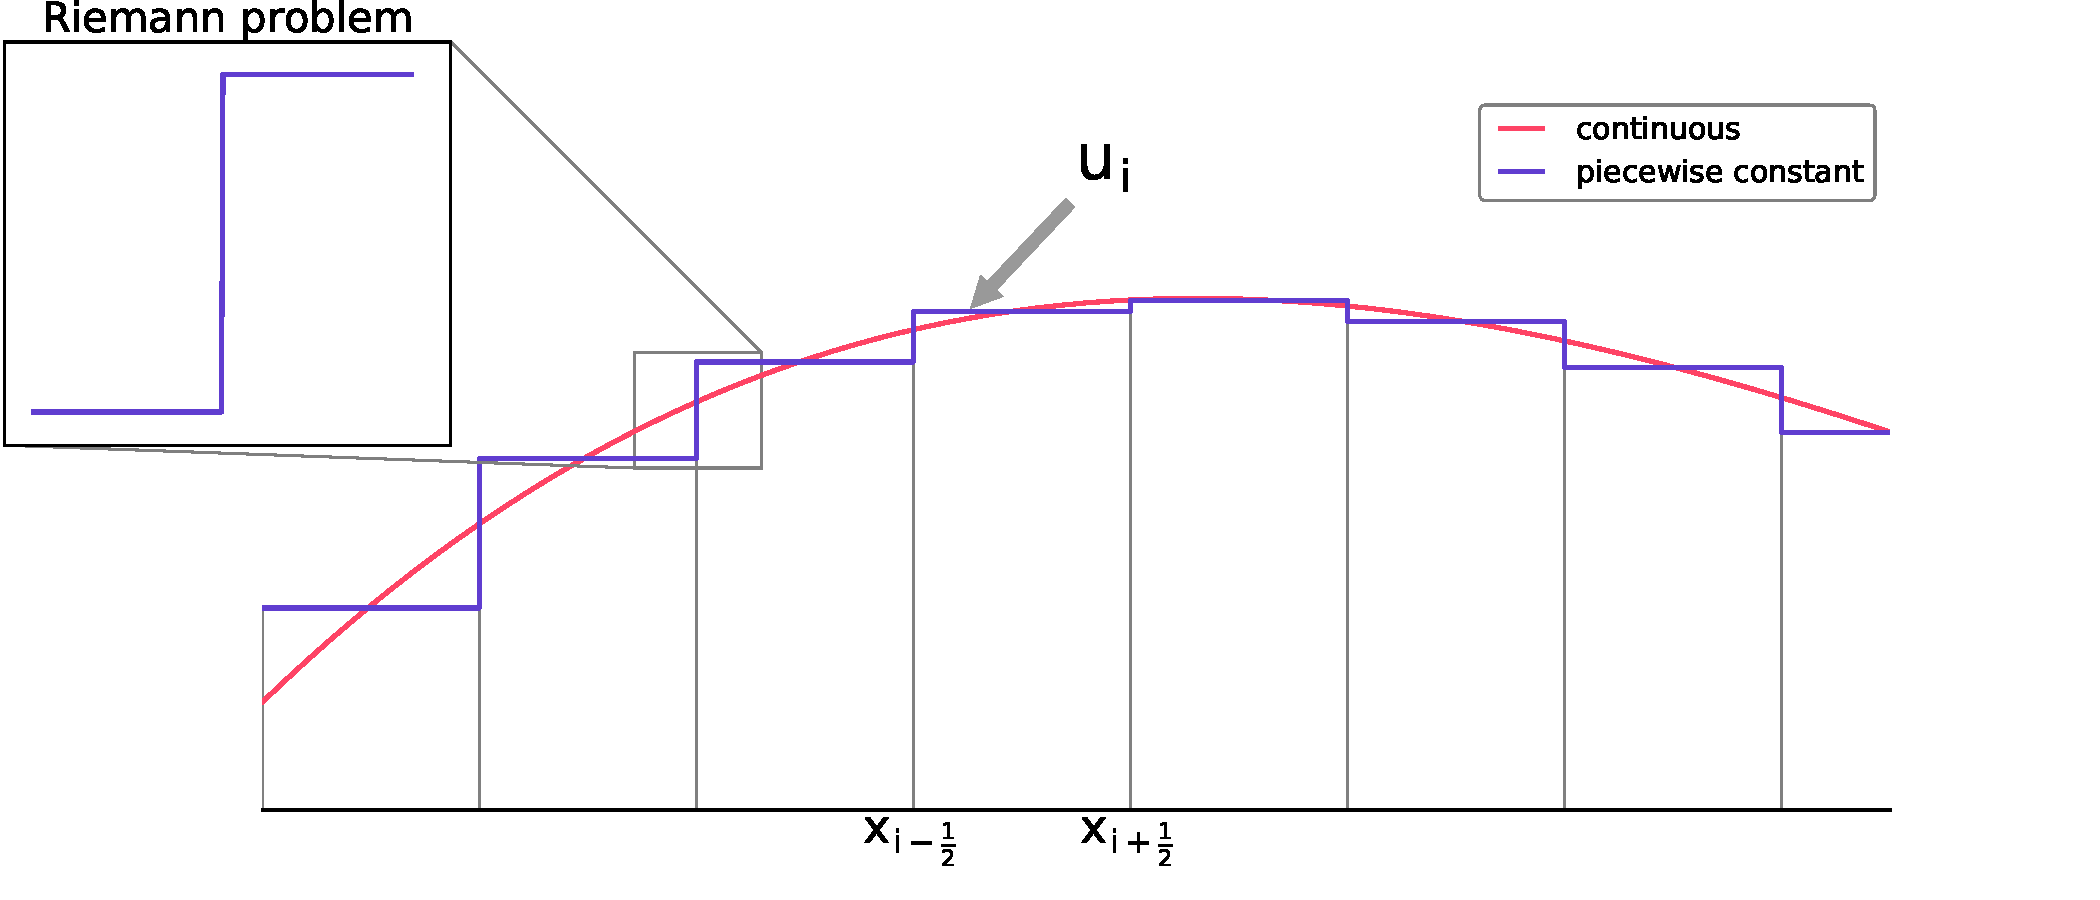
\includegraphics[width=\textwidth]{Figures/piecewise_u}
 \captionsetup{justification=justified,singlelinecheck=false,width=\linewidth}
 \decoRule
 \caption[Piecewise constant function]{A schematic example of the discretization strategy used in finite volume methods.
                                       The continuous function is averaged over the grid cells, resulting in a piecewise constant function, which is stored in memory and used to reconstruct the fluxes in the hyperbolic conservation law.
                                       Each discontinuity at the cell boundaries $x_{i-\frac{1}{2}}, x_{i+\frac{1}{2}}$ etc., describes an individual Riemann problem.}
 \label{fig:Piecewise}
\end{figure}

Inserting Eqs.~\eqref{eq:lhs} and \eqref{eq:rhs} into \eqref{eq:Finite_volume} reads

\begin{equation}
  \frac{\partial u_{i}}{\partial t} =  - \frac{1}{\vert\Omega_{i}\vert} \big(f(u_{i}, u_{i+1}) - f(u_{i}, u_{i-1})\big)
\end{equation}

The complete integral form of this partial differential equation \eqref{eq:1D_Advection} is obtained by another integration in time, propagating the state $u_{i}$ at time $t^{n}$ by a time step $\Delta t = t^{n+1} - t^{n}$

\begin{equation}
  u_{i}(t^{n+1}) - u_{i}(t^{n}) = -\frac{1}{\Delta t} \int_{t^{n}}^{t^{n+1}} \frac{\Delta t}{\vert\Omega_{i}\vert} \big(f(u_{i}, u_{i+1}) - f(u_{i}, u_{i-1})\big)\,\mathrm{d}t
\end{equation}

The above equation is often rewritten in a more algorithmic notation, with upper indices as time step reference and lower indices as cell reference

\begin{equation}
  u_{i}^{n+1} = u_{i}^{n} - \frac{\Delta t}{\Delta x} (f^{n+1/2}_{i+1/2} - f^{n+1/2}_{i-1/2})
\label{eq:Godunov_step}
\end{equation}

where $\vert\Omega_{i}\vert = \Delta x$ is the cell size, $u_{i}$ constant within the cell, and $f^{n+1/2}_{i\pm1/2}$ denotes the flux through the cell boundaries between cell $i$ and $i\pm1$, integrated over a time interval between $t^{n}$ and $t^{n+1}$.
This notation underlines the conservative properties of the equation; in words, the quantity entering through a neighboring cell and the quantity leaving the cell, amount to the change in the quantity itself.
\\[6pt]
%
% Godunov introduction ----------------------------------------------------------------------------------------
It was \citet{Godunov_1959} who first described this kind of finite volume method.
His original scheme uses the analytical solution of the \textit{Riemann problem} which occurs at each cell interface as shown in \figref{fig:Piecewise} (inset), as a building block to calculate the flux terms for \eqnref{eq:Godunov_step}; more in \secref{subsec:Riemann_problem}.
The numerical solution value is updated with the union of all exact Riemann solutions re--averaged over each cell as sketched in \figref{fig:Characteristics}.

In principle, other methods could be used to calculate the numerical flux.
An appropriate flux scheme is best chosen adjusted to the individual problem.
Overall, flux schemes can be classified either as upwind (or Godunov-type) and centered (non-upwind).
The difference between both lies in the explicit use of wave propagation information, which upwind uses, while centered schemes do not.

In the same work Godunov postulated his famous theorem which states that his scheme, and others with constant coefficients preserving monotonicity, can be at most first order accurate.
His work paved the way for many others working on non--linear, high--order schemes, resulting in many variations and extensions of the original Godunov method.


% Riemann problem ----------------------------------------------------------------------------------------
\subsection{Riemann problem}
\label{subsec:Riemann_problem}

A Riemann problem describes an initial value problem for conservation laws like \eqnref{eq:1D_Advection} involving a discontinuity in between two constant regions; see \figref{fig:Piecewise} (inset).
With a discontinuity at $x = 0$ the problem reads

\begin{equation}
  u(x, 0) = \left\{\begin{array}{l l}
            &u_{L} = \text{const.} \hspace{1cm} \text{if} \quad x\leq0\\
            &u_{R} = \text{const.} \hspace{1cm} \text{if} \quad x>0,
            \end{array} \right.
\end{equation}

where $u_{L}$ and $u_{R}$ describe the initial conditions on either side of the discontinuity.
By nature, a variable transform $x' \to cx$ and $t' \to ct$ with $c>0$ preserves the form of the conservation law, such that

\begin{equation}
  u(x, t) = u(\frac{x}{c}, \frac{t}{c}) = u(\frac{x}{t}, 1) \quad \text{for }\,t>0
\end{equation}

This shows that the solution of the Riemann problem is self-similar along constant rays of $\frac{x}{t} = c$, also called characteristics as illustrated in \figref{fig:Characteristics}.

The Godunov flux $f_{i-\frac{1}{2}}$ at $t = 0$  results from an evaluation of $u_{i-\frac{1}{2}}(\frac{x}{t})$ at $\frac{x}{t} = 0$ along the $t$-axis.

\begin{figure}[ht]
 \centering
 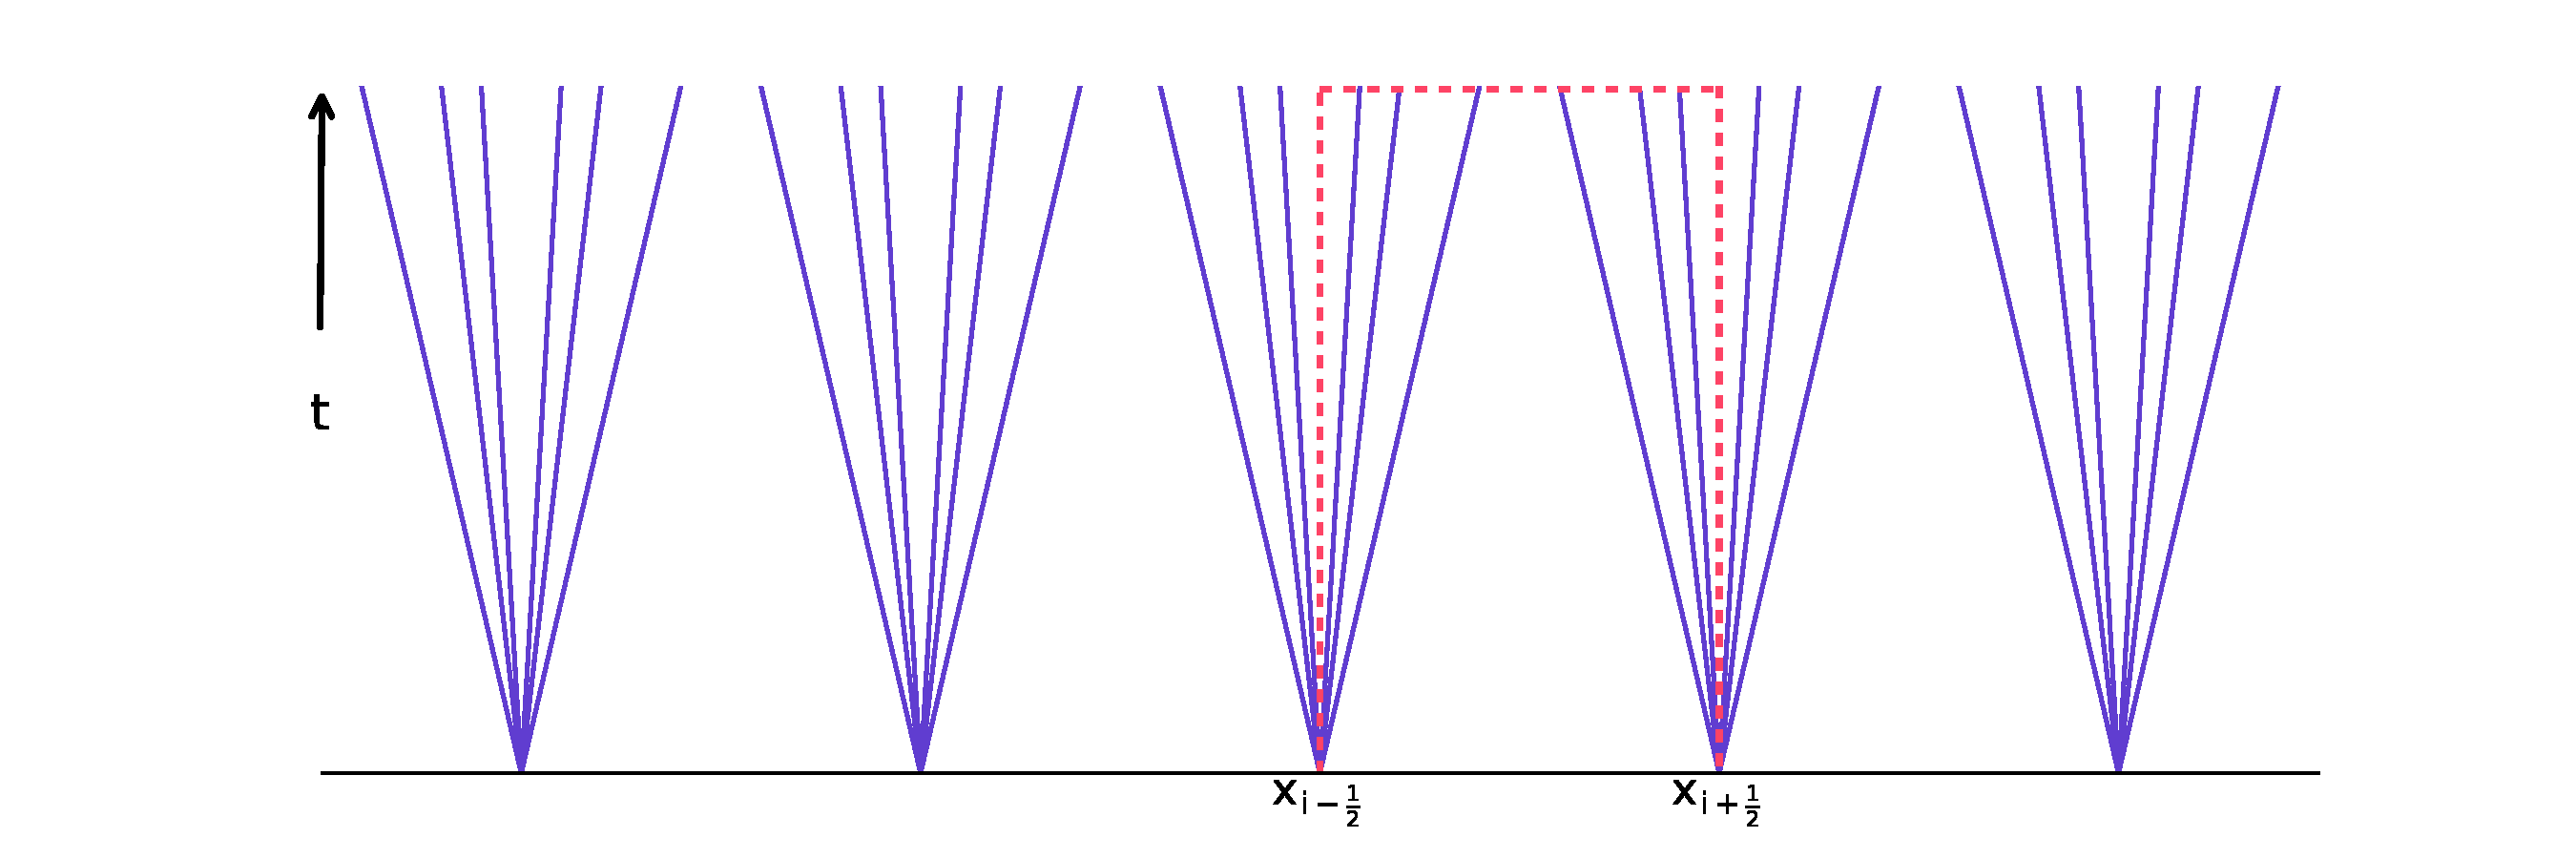
\includegraphics[width=\textwidth]{Figures/characteristics}
 \captionsetup{justification=justified,singlelinecheck=false,width=\linewidth}
 \decoRule
 \caption[Characteristics in Godunov's scheme]{Plot of the characteristics \textit{expansion fans} (blue) of the Riemann problem at each cell interface corresponding to the same discretization as presented in \figref{fig:Piecewise}.
                                               The average of the physical solutions is used to calculate the fluxes in Godunov's scheme (red).}
 \label{fig:Characteristics}
\end{figure}

In its so--called primitive form the conservation law reads

\begin{equation}
  \frac{\partial u}{\partial t} + c\cdot\frac{\mathrm{d}u}{\mathrm{d}x} = 0
\label{eq:Primitive_form}
\end{equation}

with $c=\frac{\partial f}{\partial u}$.
We can reconstruct the Godunov fluxes after an infinitesimal amount of time by using the analytical solution for the Riemann problem as described above.
Therefore we have to consider two cases: (i) $u_{L} > u_{R}$ and (ii) $u_{R} > u_{L}$, yielding the flux

\begin{equation}
  f(u_{L}, u_{R}) = \left\{\begin{array}{l l}
                    &\underset{u_{L}>u>u_{R}}{\text{max}}\big\{f(u)\big\} \hspace{1cm} \text{if} \quad u_{L}>u_{R}\\
                    &\,\underset{u_{L}<u<u_{R}}{\text{min}}\big\{f(u)\big\} \hspace{1cm} \text{if} \quad u_{L}<u_{R}
                    \end{array} \right.
\end{equation}

Since this solution has to be evaluated for every cell interface at every time step, it makes the most computationally expensive task of the whole Godunov method.

Thus, to simplify the process and reduce overhead, Riemann solvers often settle for approximations.
In the following, a few important approximative solvers are mentioned.
\\[6pt]
%
% Roe ----------------------------------------------------------------------------------------
\citet{Roe} for example writes the conservation law, or rather a whole system of conservation laws, in its primitive form as in \eqnref{eq:Primitive_form}, recovering a quasi--linear system with the Jacobian $c=\frac{\partial f}{\partial u}$.
He proceeds by locally replacing $c$ with a piecewise constant matrix for each interval $\tilde{c}(u_{L}, u_{R})$ satisfying the conditions that $\tilde{c}(u_{L}, u_{R})$ (i) is diagonalizable with real eigenvalues, (ii) is consistent with c(u) when $u_{L}, u_{R} \to u$, and (iii) conservative in the flux difference $f(u_{L}) - f(u_{R}) = \tilde{c}(u_{L}, u_{R})\,(u_{L} - u_{R})$.
This way, he achieves linearization of the system.
The flux difference thus depends on the eigenvalues, eigenvectors and characteristics of $\tilde{c}(u_{L}, u_{R})$.
The total flux is then approximated with the so--called upwinding central flux scheme $f_{i-\frac{1}{2}} = \frac{1}{2}(f_{i-1} + f_{i})$, adding these flux difference components.
\\[6pt]
%
% Osher ----------------------------------------------------------------------------------------
Similarly, Osher adds an approximation for $c$ (in \eqnref{eq:Primitive_form}) to the upwinding central flux scheme.
While Roe uses the discontinuities to approximate the Riemann solution, Osher uses $\vert c(u)\vert$, integrated on $u_{R}$ to $u_{L}$ intervals in phase space over simple wave solutions $\int_{u_{R}}^{u_{L}}\vert c(u)\vert\,\mathrm{d}u$; see \citet{Osher_Engquist, Osher_Solomon}.
\\[6pt]
%
% HLL/HLLC ----------------------------------------------------------------------------------------
The approach of \citet{HLL} (HLL hereafter) uses an even simpler approximation.
Whereas Roe and Osher approximate solutions with $N$ intermediate states for a system of $N$ conservation laws, they proposed an approximation of the Riemann solution consisting of two waves separated by three constant states.

\begin{figure}[ht]
 \centering
 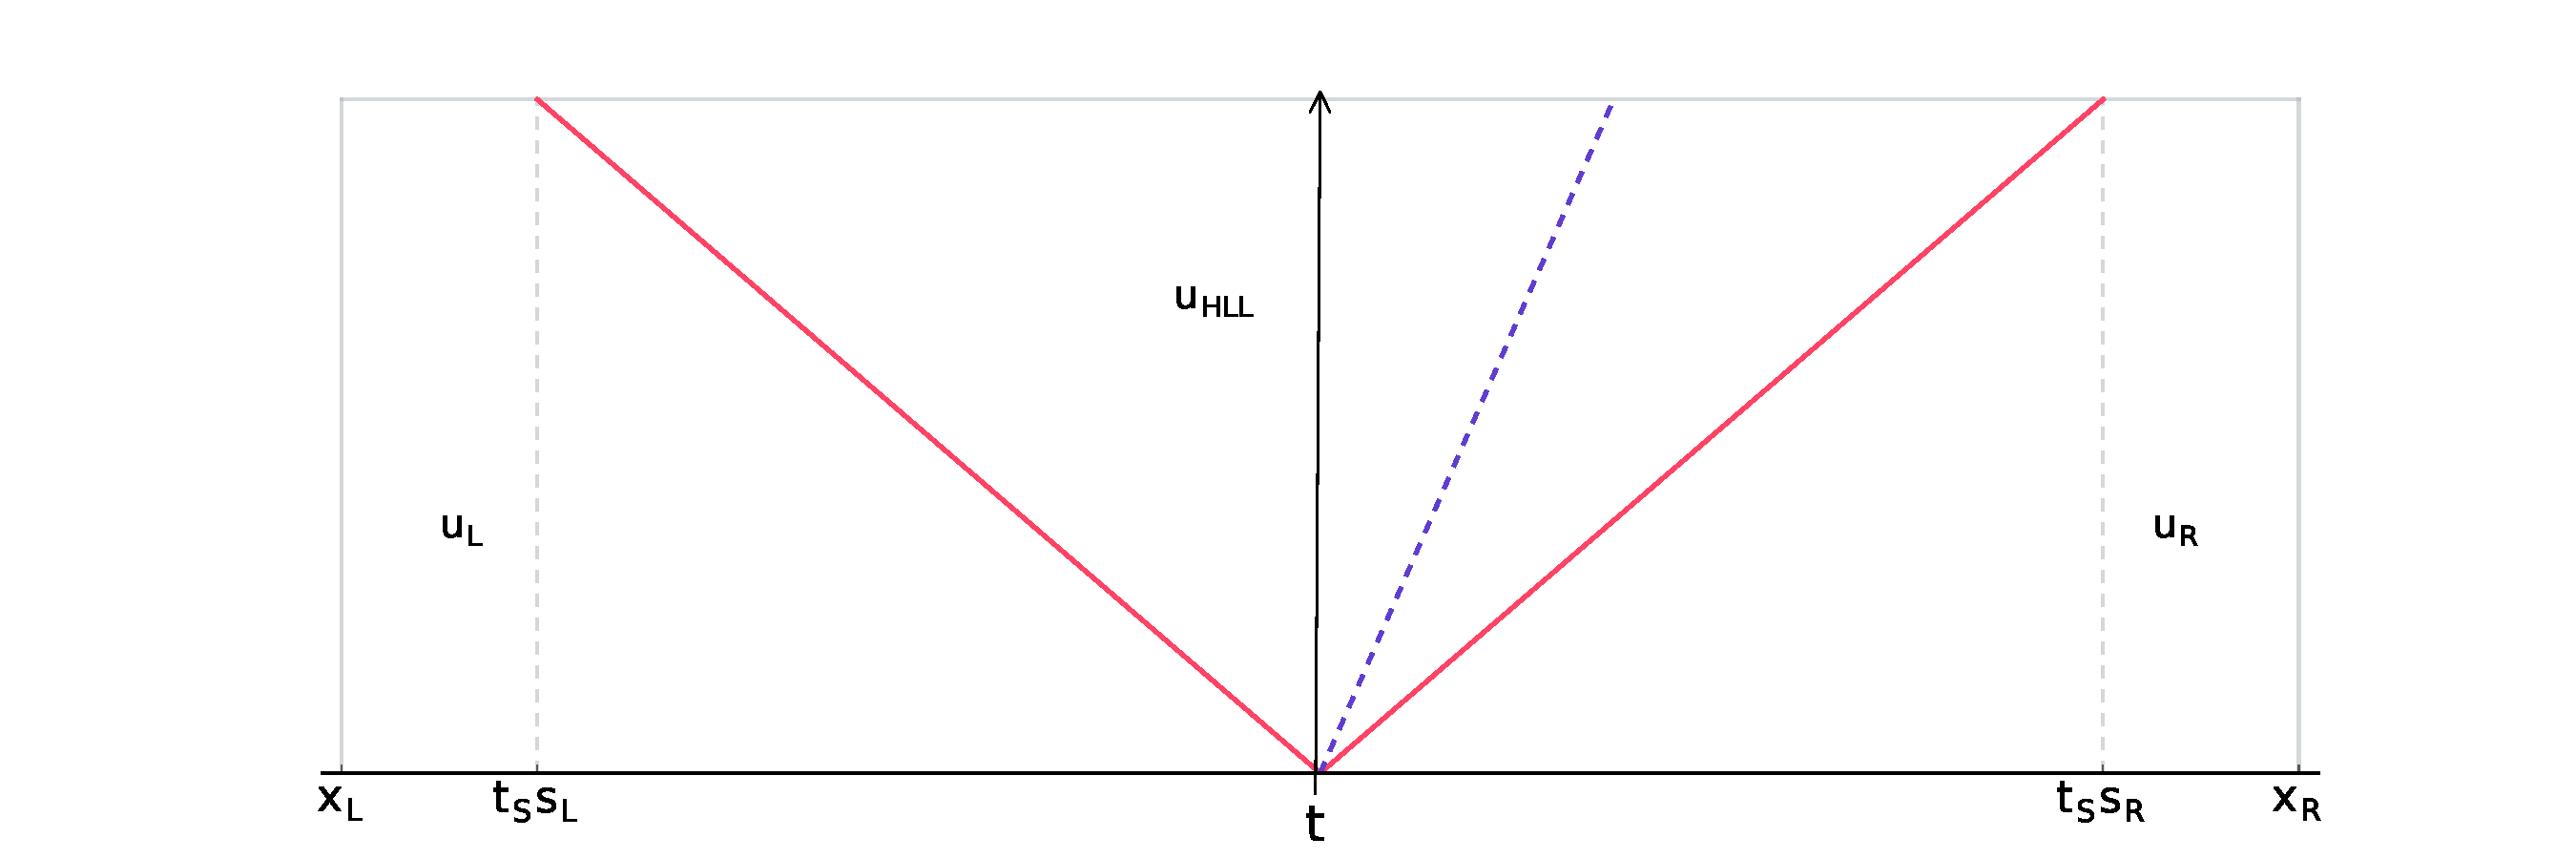
\includegraphics[width=\textwidth]{Figures/hll_regions}
 \captionsetup{justification=justified,singlelinecheck=false,width=\linewidth}
 \decoRule
 \caption[Volume partition in HLL]{The smallest and largest speeds at time $t_{s}$ divide the control volume $[x_{L}, x_{R}]\times[0, t_{s}]$ into three regions.
                                  Here, the limiting characteristics (red) are shown in an $x$--$t$ plot with an example characteristic (blue) in the $u_{HLL}$ state.}
 \label{fig:HLL_regions}
\end{figure}

Choosing a time $t_{s}>0$ the characteristics with speeds $s_{L}$ and $s_{R}$ divide a control volume $[x_{L}, x_{R}]\times[0, t_{s}]$ into three regions according to \figref{fig:HLL_regions} with

\begin{equation}
  x_{L} \leq t_{s}s_{L}\,;\qquad x_{R} \geq t_{s}s_{R}
\end{equation}

where $s_{L}$ and $s_{R}$ are the smallest and largest speeds of a signal resulting from the solution of the Riemann problem.

On this volume the integral form of the conservation law reads

\begin{equation}
  \int_{x_{L}}^{x_{R}} u(x, t_{s})\,\mathrm{d}x = \int_{x_{L}}^{x_{R}} u(x, 0)\,\mathrm{d}x + \int_{0}^{t_{s}} \big(f(u(x_{L}, t)) - f(u(x_{R}, t))\big)\,\mathrm{d}t
\label{eq:Integral_form}
\end{equation}

The integral on the left hand side split into these three regions also yields

\begin{align}
  \int_{x_{L}}^{x_{R}} u(x, t_{s})\,\mathrm{d}x &= \int_{x_{L}}^{t_{s}s_{L}} u(x, t_{s})\,\mathrm{d}x + \int_{t_{s}s_{L}}^{t_{s}s_{R}} u(x, t_{s})\,\mathrm{d}x + \int_{t_{s}s_{R}}^{x_{R}} u(x, t_{s})\,\mathrm{d}x \\
  &= (t_{s}s_{L} - x_{L}) u_{L} + \int_{t_{s}s_{L}}^{t_{s}s_{R}} u(x, t_{s})\,\mathrm{d}x + (x_{R} - t_{s}s_{R}) u_{R}
\label{eq:Integral_split}
\end{align}

Comparing \eqnref{eq:Integral_form} and \eqref{eq:Integral_split}, evaluating the flux integrals with $f_{L,R} = f(u(x_{L,R}, t_{s}))$, and dividing by the width of the wave system of the solution of the Riemann problem between the slowest and the fastest signal $t_{s}(s_{R} - s_{L})$, gives

\begin{equation}
  u_{HLL} \equiv \frac{1}{t_{s}(s_{R} - s_{L})}\int_{t_{s}s_{L}}^{t_{s}s_{R}} u(x, t_{s})\,\mathrm{d}x = \frac{s_{R}u_{R} - s_{L}u_{L} + f_{L} - f_{R}}{s_{R} - s_{L}}
\label{eq:u_HLL}
\end{equation}

The approximate solution to the Riemann problem is therefore defined over this intermediate state $u_{HLL}$.

\begin{equation}
  \tilde{u}(x, t) = \left\{\begin{array}{l l l}
            u_{L} \hspace{1cm} &\text{if} \quad \frac{x}{t}\leq s_{L}\\
            u_{HLL} \hspace{1cm} &\text{if} \quad s_{L}\leq\frac{x}{t}\leq s_{R}\\
            u_{R} \hspace{1cm} &\text{if} \quad \frac{x}{t}\geq s_{R}
            \end{array} \right.
\end{equation}

The corresponding HLL inter--cell flux is then given by the above solution for $\frac{x}{t} \to 0$ same as for the Godunov flux.

\begin{equation}
  f_{HLL} = \left\{\begin{array}{l l l}
            f_{L} \hspace{1cm} &\text{if} \quad 0\leq s_{L}\\
            \frac{s_{R}f_{L} - s_{L}f_{R} + s_{R}s_{L}(u_{R} - u_{L})}{s_{R} - s_{L}} \hspace{1cm} &\text{if} \quad s_{L}\leq 0 \leq s_{R}\\
            f_{R} \hspace{1cm} &\text{if} \quad 0\geq s_{R}
            \end{array} \right.
\end{equation}

It should be noted that the intermediate state $u_{HLL}$ is the mean value of the exact Riemann solution (by definition, see \eqnref{eq:u_HLL}), and if $u_{L}$ and $u_{R}$ are connected by a shock, the correct shock speed is obtained and the solution is exact.

\citet{HLLC} modified the HLL scheme by using an approximate Riemann solution of three waves resulting in two intermediate states, naming it the HLLC scheme.
This way, they achieve the restoration of contact surfaces and shear waves in the Euler equations.

The estimates for the signal wave speeds $s_{L}$ and $s_{R}$ remain to be determined.
They may be evaluated directly over the exact Riemann solution.
Another possibility is to use the averaged eigenvalues of Roe's as estimates.
Or the minimal eigenvalues from the left state and the maximal eigenvalue from the right state could be used to determine $s_{L}$ and $s_{R}$.
The easiest way however is to use the global, maximal signal speed of the simulation on both sides of the discontinuity with corresponding signs (e.g., $s_{L}\equiv-c$ and $s_{R}\equiv c$).
This method is called \textit{global Friedrich--Lax scheme} (GFL hereafter), for which the flux term is finally described by

\begin{equation}
  f_{GFL} = \frac{f_{L}+f_{R}}{2} - c\frac{u_{R}-u_{L}}{2}
\end{equation}


% Numerical diffusion ----------------------------------------------------------------------------------------
\subsection{Numerical diffusion}
\label{subsec:Numerical_diffusion}

The hydrodynamical Euler equations are a set of idealized conservation laws and do thus not describe realistic, physical behavior of a fluid.
They are only valid in the equilibrium state and to obtain a more realistic description, a perturbative treatment leading to higher--order corrections would be needed.

Fortunately, the Godunov scheme (using the GFL method) casts the ideal conservation laws into a modified form.
This is similar to using an infinite Taylor expansion of the conservation law in the finite difference scheme.
Since numerical methods do not work with infinite series~\footnote{unless they converge, which is unlikely}, we have to cut the Taylor expansion at some point.
This introduces a truncation error, often referred to as \textit{numerical diffusion}.
The 'actual' equation solved by the Godunov scheme is a combination of a hyperbolic and a parabolic partial differential equation.

\begin{equation}
  \frac{\partial\textbf{U}}{\partial t} + \nabla\cdot\textbf{F} = \nu_{num}\Delta\textbf{U}
\end{equation}

In GFL this numerical diffusion coefficient $\nu_{num} = \frac{c\Delta x}{2}$ is maximal (for hydrodynamics usually estimated with the sound speed $c_{s}$ as $c = \mathrm{max}\big\{ \vert v_{L}\vert + c_{s}, \vert v_{R}\vert + c_{s} \big\}$).
It is desirable to minimize the truncation error as much as possible, although without any numerical diffusion at all the time integration becomes unstable.


% MUSCL ----------------------------------------------------------------------------------------
\section{MUSCL scheme}
\label{sec:MUSCL}

% Godunov advantages ----------------------------------------------------------------------------------------
The advantage of a Godunov--type scheme is the clear physical picture, it is built on.
Instead of replacing an infinite Taylor series with a truncated one, it conforms a complexly structured physical system to a simple data representation.
This data is exactly evolved for a time step.
The result is then re--simplified similarly as before, preparing it for the next temporal propagation.

However, Godunov himself proved that stable, linear schemes achieve at most first order accuracy.
Hence it can be very diffusive and smearing around discontinuities.
On the other hand, higher order classical schemes which produce sharper discontinuities, but also spurious oscillations around them, possibly attain unphysical values.

From a physical point of view, it is thus immensely appealing to use a Godunov-type scheme's advantages and still carry the accuracy of the data description to higher orders to gain structural resolution.
\\[6pt]
%
% Piecewise linear ----------------------------------------------------------------------------------------
This is achieved by changing the averaging of cell states by moving from a piecewise constant function to another function, say a piecewise linear function as depicted in \figref{fig:Piecewise_linear}.
Such type of method is called MUSCL scheme (Monotonic Upstream--centered Scheme for Conservation Laws), although it was originally the name of P. Woodward's program incorporating B. van Leer's ideas.
There are approaches which extend the idea even further and replace it by a piecewise parabolic function; see \citet{PPM_Colella}.

The new description of the data representation could look something like

\begin{equation}
  u_{i}(x) = \bar{u}_{i} + \frac{\Delta_{i} u}{\Delta x} (x - x_{i})
\end{equation}

where $\bar{u}_{i}$ is the piecewise constant value from the Godunov scheme, $x_{i}$ the center coordinate of the cells, $\Delta x$ the cell size, and $\frac{\Delta_{i} u}{\Delta x}$ the slope, which remains to be determined.

There were several proposals from \citet{MUSCL_1, MUSCL_2} how to express the slope

\begin{itemize}
  \item either the Godunov averaged cell values $\Delta_{i} u = \frac{1}{2}(u_{i+1} - u_{i-1})$
  \item or the difference of the underlying continuous function $\Delta_{i} u = u(x_{i+\frac{1}{2}}, t) - u(x_{i-\frac{1}{2}}, t)$ at the cell interfaces
  \item or using a combination like $\Delta_{i} u = \frac{12}{(\Delta x)^{2}}\int_{x_{i-\frac{1}{2}}}^{x_{i+\frac{1}{2}}} u(x, t) (x - x_{i}) dx$
\end{itemize}

\begin{figure}[ht]
 \centering
 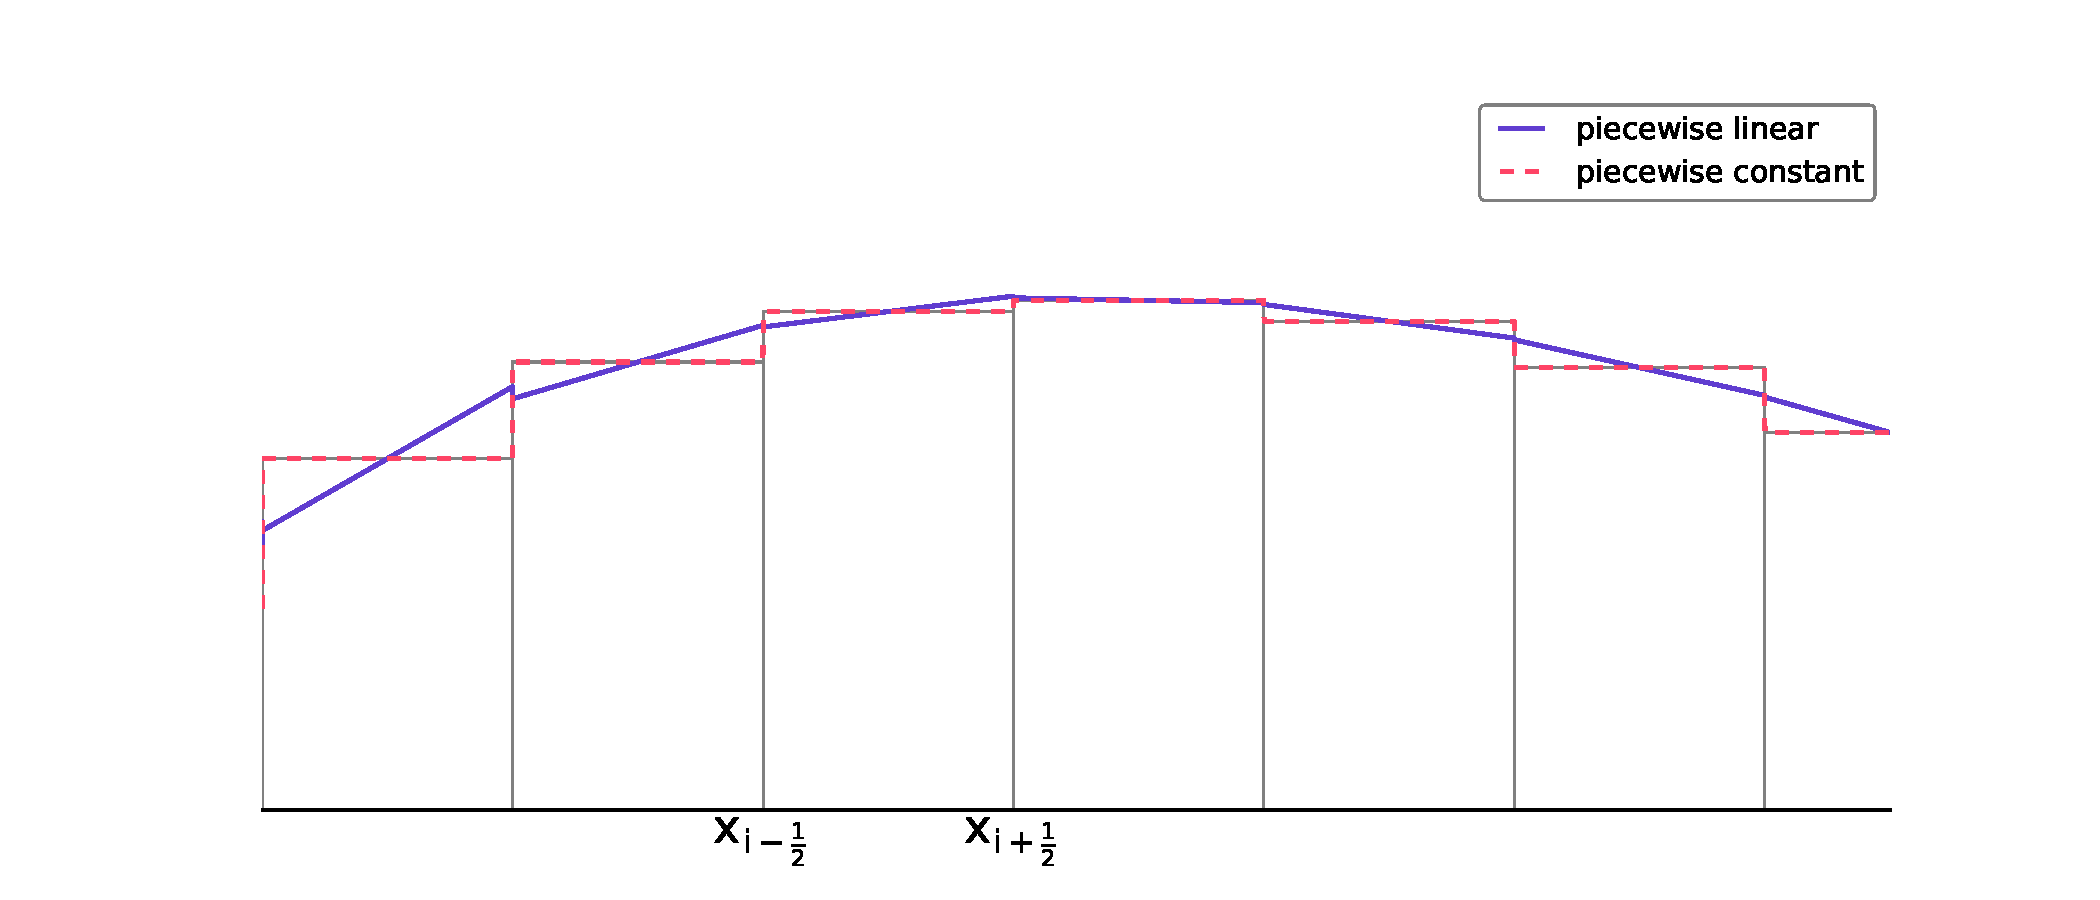
\includegraphics[width=\textwidth]{Figures/pw_linear}
 \captionsetup{justification=justified,singlelinecheck=false,width=\linewidth}
 \decoRule
 \caption[Piecewise linear function]{A schematic example of the extension from first order Godunov scheme to higher orders.
                                     The piecewise constant data representation is replaced by a piecewise linear function, moving up from first order to higher accuracy.}
 \label{fig:Piecewise_linear}
\end{figure}

These lift the accuracy up to second order.
However, there is a catch to changing the data representation, which often renders the method unstable.

% TVD ----------------------------------------------------------------------------------------
To make possible problems more evident, we consider a property of discretization schemes introduced by \citet{Harten_TVD}.
The discretized total variation is

\begin{equation}
  TV(u) = \sum_{i} \vert u_{i} - u_{i-1}\vert
\end{equation}

If the total variation decreases or at least stays the same with time steps, i.e. $TV(u^{n+1}) \leq TV(u^{n})$, the scheme is called \textit{total variation diminishing} (TVD hereafter).
Harten proved that numerical schemes are called \textit{monotonicity preserving} if they are TVD and vice versa.

To outline differences between piecewise constant and piecewise linear schemes, we consider an underlying analytical function with local extrema.
The piecewise constant data representation of the underlying function generally underestimates the absolute value of local extrema provided sufficient spatial resolution.
In the case of a piecewise linear scheme it is possible that the values are overestimated assuming the curvature around the extrema is relatively high.
This causes non--physical oscillations with growing amplitudes around the extrema, rendering the scheme potentially unstable.
Such oscillations increase the total variation, thereby breaking the TVD property.
As follows, total variation evidently makes an excellent monitor of a scheme's oscillatory behavior.
Thus, a monotonicity preserving scheme of higher order is desirable.
\\[6pt]
%
% slope delimiters ----------------------------------------------------------------------------------------
To preserve monotonicity in otherwise monotonicity destroying schemes, but to still profit of higher order strategies, \textit{slope limiters} are introduced.
As the name gives away, they define a limit for the slope of $u$ beyond which the improving scheme is locally reverted back to a piecewise constant scheme, i.e. with a slope equal to zero.

\citet{vanLeer_fluxlimiter} defined his symmetrically monotonized central slope limiters (MonCen hereafter) as

\begin{equation}
  (\Delta_{i} u)_{\text{MonCen}} = \left\{\begin{array}{l l}
                                    \text{sgn}(\Delta_{i} u)\text{min}\big\{ 2\vert\Delta u_{i-\frac{1}{2}}\vert, \vert\Delta_{i} u\vert, 2\vert\Delta u_{i+\frac{1}{2}}\vert \big\} \hspace{1cm} & \text{if} \quad \text{sgn}(\Delta u_{i-\frac{1}{2}}) = \text{sgn}(\Delta u_{i+\frac{1}{2}}) \\
                                    0 \hspace{1cm} &\text{otherwise}
                                   \end{array}\right.
\end{equation}

where $\Delta u_{i\pm\frac{1}{2}} = \pm(u_{i} - u_{i\pm1})$ are the slopes to the left, resp. right side.
These limiters prevent the slope to exceed the range of values of neighboring cell averages
Would the slope take values outside the range between the limits, it instead reverts to the first order description.
This way monotonicity is preserved by excluding the problematic cases.
The limits work for any of the choices for $\Delta_{i} u$ from above.

For the first choice of slope the limiter can be written as

\begin{equation}
  \phi_{VL}(r_{i}) = \frac{r_{i} + \vert r_{i}\vert}{1 + \vert r_{i}\vert}
\end{equation}

where $r_{i} \equiv \frac{u_{i-\frac{1}{2}}}{u_{i+\frac{1}{2}}} = \frac{u_{i} - u_{i-1}}{u_{i+1} - u_{i}}$ is the ratio of slopes on the left and the right.
Unfortunately, in certain situations the MUSCL scheme is still unstable with MonCen limiters.

Another much less aggressively restrictive strategy is the MinMod limiter by Roe; see \citet{Sweby}.

\begin{equation}
  (\Delta_{i} u)_{\text{MinMod}} = \left\{\begin{array}{l l}
                                   \text{min}\big\{ \vert\Delta u_{i-\frac{1}{2}}\vert, \vert\Delta u_{i+\frac{1}{2}}\vert \big\} \hspace{1cm} & \text{if} \quad \text{sgn}(\Delta u_{i-\frac{1}{2}}) = \text{sgn}(\Delta u_{i+\frac{1}{2}}) \\
                                   0 \hspace{1cm} &\text{otherwise}
                                   \end{array}\right.
\end{equation}

If the signs of the slopes on the left and right are the same, the one with the minimal modulus is chosen, otherwise the scheme locally reverts to first order.

With any higher order Godunov--extension scheme, the Riemann problems have to be generalized.
States flanking the discontinuity due to the particular discretization strategy are not constant anymore.
This breaks the self-similarity of the constant Riemann problem, thereby causing the characteristics to bend.
The flux cannot be described by \eqnref{eq:rhs}, which makes exact flux reconstruction harder.
In this case, a predictor step is usually used to approximate the values of the conserved quantities at cell edges at $t+\Delta t/2$.
These predicted values are then used to non--linearly reconstruct the fluxes and update the solution to $t+\Delta t$.
By doing so, a higher--order reconstruction is used for a linear scheme, which does not violate Godunov's theorem.

There are many schemes carrying the idea of extending the Godunov method even further, making modifications in many aspects.


% Source terms  ----------------------------------------------------------------------------------------
\section{Source terms}
\label{sec:Source_terms}

Traditionally source terms refer to inhomogeneous contributions in (hyperbolic) partial differential equations, as in \eqref{eq:Conservation_law}.
So far these terms have been ignored for sake of simplicity.

Sometimes it is appropriate to write the source term as a relaxing deviation from an equilibrium state

\begin{equation}
  \textbf{S}(\textbf{U}) = \frac{\textbf{U}_{eq} - \textbf{U}}{t_{relax}}
\end{equation}

where $\textbf{U}_{eq}$ is the equilibrium state, such that $\textbf{S}(\textbf{U}) \to 0$ for $\textbf{U} \to \textbf{U}_{eq}$, and $t_{relax}$ of the order of a relaxation time scale.
%This can be approximated with the characteristic linear slope of the source term.
%
% \begin{equation}
%   t_{relax} = \big(\mathrm{Tr}(\frac{\partial\textbf{S}}{\partial\textbf{U}})\big)^{-1}
% \end{equation}

With the Godunov solver (especially simple with GFL) we associate another intrinsic time scale, determined by the so--called \textit{Courant factor}

\begin{equation}
  \Delta t = \frac{\Delta x}{c}
\end{equation}

where $c$ is the maximal signal speed in the characteristics associated to a Riemann problem.

Incorporating the source term with the 'homogeneous' Godunov solver is therefore only possible in certain situations.
If the Godunov time scale is smaller than the relaxation time, $t_{relax} > \Delta t$, then the process of the homogeneous part of the conservation law (e.g. the hydrodynamical flow) is much faster compared to the physical process given by the source term.
If on the other hand $t_{relax} < \Delta t$, the source term needs to be carefully coupled to the homogeneous part.
If so, the source term is called \textit{stiff}.
\\[6pt]
%
In the non--stiff regime the most common method to solve hyperbolic partial differential equations with source terms is the \textit{operator--splitting approach}.
Its basic idea is to use fractional steps, splitting the full non--homogeneous conservation law into the homogeneous equation supplemented by the ordinary differential equation

\begin{equation}
  \frac{\mathrm{d}\textbf{U}}{\mathrm{d}t} = \textbf{S}(\textbf{U})
\end{equation}

alternatively solving one then the other equation within a full time step.
First a temporary state is calculated with the previously mentioned Godunov scheme.

\begin{equation}
  \textbf{U}^{n+\frac{1}{2}} = \textbf{U}^{n} - \Delta t \nabla \cdot \textbf{F}(\textbf{U}^{n})
\end{equation}

In an explicit time step the temporary state is used to account for the source term.

\begin{equation}
  \textbf{U}^{n+1} = \textbf{U}^{n+\frac{1}{2}} + \Delta t \textbf{S}(\textbf{U}^{n})
\end{equation}

If the source term tends to stiffness, a much more suited implementation of the source term is an implicit time step, in which the source term depends on the solution of the following time step.

\begin{equation}
  \textbf{U}^{n+1} = \textbf{U}^{n+\frac{1}{2}} + \Delta t \textbf{S}(\textbf{U}^{n+1})
\end{equation}

This obviously complicates the calculation.
Solving for the still unknown solution $\textbf{U}^{n+1}$ then often requires iterative Newton--Raphson root finding algorithms for possibly, highly non-linear terms and fast approximators for the Jacobian which is required for the algorithm.

In the particular case when the source term describes heating and cooling functions, the implicit source--term--related time step is often referred to as \textit{thermochemistry step}.
If the Newton--Raphson algorithm in this case does not converge, one commonly resorts to a subcycling method.
Herein the time step is again split into a number of substeps with the condition that the final result does not increase more than up to a predefined limit.
This limit is usually defined over the factor of $0.1$, accordingly called the \textit{10\% rule}.

\begin{equation}
  \vert \textbf{U}^{n+1}-\textbf{U}^{n}\vert \leq 0.1\times\textbf{U}^{n}
\end{equation}

With these methods the strict conservation of the state variables may not apply anymore.
If this is of special interest, there is almost no choice left, but to directly include the source term in the Godunov scheme in a single implicit time step, thereby leaving the operator--splitting approach.

\begin{equation}
  \textbf{U}^{n+1} = \textbf{U}^{n} - \Delta t \nabla \cdot \textbf{F}(\textbf{U}^{n+1}) + \Delta t \textbf{S}(\textbf{U}^{n+1})
\end{equation}

\citet{LeVeque_source_balancing} proposed an alternative approach to deal with source terms which he called \textit{source--balancing}.
His basic idea was to introduce another discontinuity in the center of each cell through a decomposition of the piecewise constant values into $\textbf{U}_{i}^{-}$ and $\textbf{U}_{i}^{+}$.
If somehow possible, this should be done conservatively such that

\begin{equation}
  \textbf{F}(\textbf{U}_{i}^{+}) - \textbf{F}(\textbf{U}_{i}^{-}) = \Delta x\textbf{S}(\textbf{U}_{i})
\end{equation}

If the decomposition was chosen appropriately, as a consequence the source term in the cell is exactly canceled by the newly introduced Riemann problem.
The source term can therefore be excluded in the Godunov solver, which now simply has doubled workload.
\\[6pt]
%
How to deal with source terms and their stiffness is of course also dependent on the individual problem at hand.
In the following, some important source term versions are briefly discussed.


% Gravitational source terms  ----------------------------------------------------------------------------------------
\subsection{Self--gravity}
\label{subsec:Gravity_source}

The probably most important source term in astrophysics is gravity.
For a very massive group of bodies, gravity dominates over all other forces and is the bonding force, which holds the group together.
Such a group of bodies is then referred to as \textit{self--gravitating}.

Since gravity is a long--range force and practically ubiquitous, it is usually by default already accounted for in the hydrodynamical Euler equations as an external force field; see \eqnref{eq:EulerMomentum} and \eqref{eq:EulerEnergy}.
It is specified by the gravitational potential gradient which in turn is related to the mass density through the Poisson equation.

\begin{equation}
  \textbf{a} = -\nabla\phi \qquad\text{ and }\qquad \Delta\phi = 4\pi G\rho
\end{equation}

These source terms can be solved with the previously mentioned operator--splitting method.

Before the gravitational acceleration, resp.~work done by gravity, can be included in the second half of the split time step, the Poisson equation has to be solved.
This is accomplished with a standard Poisson solver using an iterative relaxation method.
Due to the fact that in physics Poisson equations are omni--present, many excellent methods have been developed over the years with the aim of providing fast and efficient solutions.

For AMR codes a natural choice is the multi--grid methods described in \citet{Multigrid_Poisson}.
It uses a hierarchy of decreasing discretization levels, for which the spatial resolution increases for each higher level.
Each of these levels require boundaries of only one--cell thickness, which may be arbitrarily complex.
This makes it especially suited for parallelization through computational domain decomposition.
Whereas others, classical methods' convergence depends on the grid size, this methods convergence properties do not.
Another advantage which distinguishes this method from others is that no initial guesses are required, since the coarsest level can be taken as initial condition.
The coarse levels' potential is then interpolated to finer levels.

Due to this hierarchical structure of the mesh grid, AMR codes often use an adaptive time stepping method which allows finer levels to subcycle coarser ones.
This can come in conflict with the Poisson solver and cause a delay effect, since finer levels are interpolated from the not--yet--advanced coarse level.
This effect is particularly noticeable in high--resolution, high--density regions.

For hydrodynamical simulations which combine gas and particle dynamics, the source density has to be prepared first.
This can be done by projecting particles onto the coarse grid using a particle shape function and adding it to the gas density.

After the Poisson solver did its work the gravitational acceleration can be easily calculated using a standard finite difference gradient operator, which is then inserted into the second half of the split time step.


% Radiation source terms  ----------------------------------------------------------------------------------------
\subsection{Radiation source terms}
\label{subsec:Radiation_source}

In computer simulations in which more than one dynamical system is being modeled, it is always important to compare the corresponding signal velocities.
This is especially crucial for the case in which radiative waves and material waves (e.g.,~molecular hydrogen) interact, because their propagation speeds differ by a factor of $\sim 150\,000$.
In the diffusion limit, mentioned in \secref{subsec:Diffusion_limit}, radiation and matter are both close to LTE and the mean free path of photons is very small.
Regarding numerical methods, it is accordingly interesting to investigate how numerical diffusion $\nu_{num}$ compares to the physical, radiative diffusion $\nu_{rad}$.

\begin{equation}
  \nu_{num} = \frac{c\Delta x}{2} \qquad\text{ and }\qquad \nu_{rad} = \frac{c\lambda}{3}
\end{equation}

In optically thick media, the mean free path $\lambda$ of a photon is very small compared to the length scale associated with the numerical scheme.~\footnote{The modified radiative energy moment equation which is actually solved by the Godunov scheme correspondingly reads
\begin{equation}
  \frac{\partial E}{\partial t} - \frac{c\lambda}{3}\Delta E - \frac{c\Delta x}{2}\Delta E = \frac{caT^{4} - cE}{\lambda}
\end{equation}
}
Consequently the numerical diffusion becomes larger than the diffusion of the radiation, and the numerical scheme inaccurate.
The source term whence becomes stiff.

To resolve this issue one has several choices.
\begin{itemize}
  \item In an AMR method there is the possibility to simply refine the grid and thereby reducing $\Delta x$.
  If this can be done often enough the inequality $\nu_{num} < \nu_{rad}$ might be reached.
  However AMR codes can only go so far and the refinement of the mesh grid might not be enough to alleviate the problem.
  \item \citet{Berthon_diff_flux} presented another method in which the Godunov flux is modified similarly to the flux, resp. slope, limiters discussed in \secref{sec:MUSCL}.
  Here, the fluxes are changed such that radiation diffusion is explicitly corrected for in the Riemann solver.
  \item Another possibility was already discussed in the last chapter in \secref{subsec:Asymptotic_limits}.
  By splitting a photon group into a streaming and a trapped subgroup, we identify the photons for which the source term becomes stiff, the trapped photon group.
  We can use the ordinary Godunov solver for the streaming photon group to perform the advection.
  The source terms for the whole photon group are then included in a thermochemistry step (see \secref{sec:Source_terms}) and coupled to the hydrodynamics.
  This way the photons are advected such that the diffusion limit is correctly accounted for.
\end{itemize}

Furthermore, if the source term is still non--stiff, the explicit time integration (in the operator--splitting method) of the radiative source term would slow down the entire simulation.
Hence an important approximation is usually applied in radiation hydrodynamics simulations, the RSLA (Reduced Speed of Light Approximation).
As the name already indicates, herein the speed of light is reduced, usually by a factor of $\sim10^{2}$ to $\sim10^{3}$.
This is only valid if the light crossing time is still short compared to the sound speed's time scale.
If the RSLA is not valid, one has to rely on the implicit time integration methods mentioned above.


% Adaptive mesh refinement  ----------------------------------------------------------------------------------------
\section{Adaptive mesh refinement}
\label{sec:AMR}

Adaptive mesh refinement was introduced by \citet{AMR_colella}.
The basic idea of the AMR technique arises quite naturally in the investigation of numerical diffusion.

As already mentioned in \secref{subsec:Numerical_diffusion}, numerical diffusion occurs due to truncation errors from a numerical scheme.
For a stable and physically accurate numerical scheme, we have to require that the numerical diffusion term is much smaller than the physical flux from the conservation law.
If the numerical diffusion becomes too large, we have to find ways to reduce it.
One way to do this is to switch to a higher--order numerical scheme.

But if we look at the the numerical diffusion coefficient (from Godunov scheme using GFL) again, perhaps another much more natural way may come to mind.

\begin{equation*}
  \nu_{num} = \frac{c\Delta x}{2} \qquad\quad\text{with}\qquad c = \mathrm{max}\big\{ \vert v_{L}\vert + c_{s}, \vert v_{R}\vert + c_{s} \big\}
\end{equation*}

It is possible to reduce numerical diffusion by simply decreasing $\Delta x$, the grid spacing.
Locally decreasing the cell size in AMR is achieved by simply partitioning it into $2^{ndim}$ smaller (evenly spaced) cells.

This mixing of different grid spacings brings complications.
The classical Godunov solver has to be adapted to more complex interface fluxes due to the varying mesh geometry.
For instance on refinement boundaries it is possible to have a flux coming from one side, and to the other side a flux leaving to more than a single cell.
Therefore, interpolations and averages are frequently employed in the adjustment of the Godunov solver to adaptive refinement, which introduces accuracy errors and might render the scheme not perfectly conservative anymore.

All this results in a \textit{refinement criterion} for the limitation of numerical diffusion.

\begin{equation}
  \epsilon_{num} < \frac{\Delta x\,\vert\Delta \textbf{U}\vert}{\vert\nabla\cdot\textbf{F}\vert}
\end{equation}

However, refinement criteria are not limited to the minimization of numerical diffusion, but can be expanded to other physical conditions one wishes to enforce.

An SPH--like strategy for example defines another refinement criterion which sets a minimal mass $M_{SPH}$ within a cell of given size.

\begin{equation}
  M_{SPH} < \rho\,(\Delta x)^{3}
\end{equation}

Especially relevant for star formation is another variant of refinement criterion

\begin{equation}
  \epsilon_{Jeans} < \frac{\Delta x}{\lambda_{J}}
\end{equation}

where $\lambda_{J}$ is the Jeans length (see \secref{subsec:Instabilities}).
If a gravitational instability occurs the cells are refined in order to better resolve the spatial scale set by the sound speed.
This can result in a problematic cascade of refinements, which is often stopped with so--called \textit{sink particles}.
\\[6pt]
%
If one of the above criteria is fulfilled, a region around the cell is locally refined.
The efficiency parameters $\epsilon_{num}$, $\epsilon_{courant}$, $M_{SPH}$, and $\epsilon_{Jeans}$ determine the aggressiveness of the refinement strategy.
Their values have to be adjusted to reach reasonable accuracy given the available computational resources.

So--called \textit{patch--based} AMR algorithms expand this region more generously in patches, whereas \textit{tree--based} algorithms interpret refinement strategies in a much smaller neighborhood.
Patches have rectangular buffer zones around the cell center in which a criterion actually triggered refinement.
Cells of these buffer zones are refined even though the criterion might have not been fulfilled individually for each.
The advantage of patches lies in the simpler form of the resulting mesh grid, which simplifies flux calculations and thereby the construction of higher--oder schemes.
Tree--based algorithms on the other hand are more conserving with computational resources and trace only physically relevant structures, provided the refinement criteria are based on physical conditions.


% RAMSES  ----------------------------------------------------------------------------------------
\section{RAMSES}
\label{sec:RAMSES}

RAMSES~\footnote{acronym for 'Raffinement Adaptatif de Mailles Sans Efforts Surhumains' --- AMR for non--superhumans} is a general hydrodynamics simulator that encompasses all the numerical methods previously mentioned in this chapter.
It is an open--source code initially created and developed by \citet{Romain_RAMSES}.~\footnote{\url{http://www.bitbucket.org/rteyssie/ramses}}
Its original purpose was to study the cosmological evolution of dark--matter under self--gravity in a large--scale context.
But over the years, it attracted a considerable group of users and contributors all over the world and its foundation was extended to satisfy each and everyones needs.
By now it provides a basic tool for astrophysical simulations involving self--gravitating hydrodynamical flows which interact with several physical components, such as magnetic fields or radiation.

The program's source code is written in the programming language \code{FORTRAN90} and includes the \code{MPI} library~\footnote{\url{http://www.mpi-forum.org/}; a standardized message passing interface designed for parallel computers} for parallel execution.
RAMSES is parallelized with a complicated domain decomposition strategy which conforms with its AMR data structures.
It is therefore capable of simultaneously running on hundreds of CPUs on high--performance, super--computing clusters.

The core modules of RAMSES can be split into 4 parts.

\begin{itemize}
  \item \code{ramses/amr/} provides AMR service routines and constructs the fundamental data structure, a \textit{fully threaded tree}; see \citet{Fully_Threaded_Tree}.
  Its basic elements are called \textit{octs} and consist of $2^{ndim}$ cells, where $ndim$ is the chosen number of dimensions (1, 2, or 3).
  These octs are assigned to different refinement grid levels $l$, which go from the coarsest base level $0$ to a definable maximum level.
  They are sorted in a double linked list, pointing to a parent cell at $l-1$, the parent's $2\times ndim$ neighboring cells, and to its children cells at $l+1$.
  The sorting is done with a \textit{Hilbert key} which is especially advantageous for parallelization purposes.
  This way routines requiring information from neighboring cells can quickly access their data.
  It also limits memory usage to 17 integers per oct (in 3 dimensions).
  \item \code{ramses/pm/} contains the Particle Mesh routines.
  It includes the description of particles, such as dark matter particles, star particles, or so--called sinks.
  The dynamics of these particles is calculated by standard grid--based N--body schemes.
  A particle belongs to a certain oct if its position fits into the oct's boundaries.
  The mass of particles is projected onto the grid using a smoothing window~\footnote{with a CIC (cloud--in--cell) interpolation scheme} to be integrated into the Poisson solver.
  \citet{Andreas_sinks} had a main contribution to the \textit{sink particle} integration to RAMSES.
  In this thesis sink particles were used to represent collapsing, accreting and luminous protostars.
  They represent point masses, whose creation is triggered if a cell mass density reaches a certain threshold.
  \item \code{ramses/poisson/} contains the Poisson solver as mentioned in \secref{subsec:Gravity_source}.
  \item \code{ramses/hydro/} contains hydrodynamics solver routines.
  The Godunov scheme builds the foundation for this module; see \secref{sec:Godunov}.
  It is upgraded to a second--order scheme using the MUSCL scheme and several flux limiter implementations, the MinMod limiter being the most stable amongst them; see \secref{sec:MUSCL}.
\end{itemize}

In order to simulate star formation an important extension to RAMSES was used.
\citet{Joki_RT, Joki_IR} implemented a radiative transfer module (\code{/ramses/rt/}), renaming it RAMSES--RT.
It couples radiative transfer with the hydrodynamics according to \chapref{sec:RadiativeTransfer} and particularly \secref{subsec:Coupling_to_HD}.
RAMSES--RT provides 3 photon groups, of which only the IR (infrared) photon group was utilized in this thesis.
With an M1 approximation for the radiative pressure tensor the diffusion limit as well as the streaming limit are relatively well resolved.


% Sink particles  ----------------------------------------------------------------------------------------
\subsection{Sink particles}
\label{subsec:Sink_particles}

RAMSES(--RT) uses so--called sink particles to represent collapsing protostars and fully grown stars.

In \secref{subsec:Larson_cores} the density threshold of an optically thick core of around $10^{-13}$ g/cc with a Jeans length of around 4 AU has been physically motivated.
Ideally, the entire collapse procedure should be computed using multi--group radiation hydrodynamics to obtain the proper behavior up to the formation of the second Larson core or even to the point when nuclear fusion is supposed to initiate in the innermost core.
However, since these simulations require very high resolution, their demand of computational resources would be enormous.

Simply replacing the collapsing object with a point mass particle after it went through the formation of the first core, therefore presents an acceptable compromise.
After its formation the sink is removed from the hydrodynamical simulation and its gravitational potential computed as a source term in the Euler equations.
This way, the sink particle formation is physically founded and simultaneously preserves valuable computational resources.

Yet, some simulations cannot even afford to resolve a length scale of 4 AU.
In this case, the sink particle is chosen to form in a Jeans length bigger than, but still as close to 4 AU as possible.
The density threshold is then determined with

\begin{equation}
 \rho_{sink} = \frac{c_{s}^{2}}{16G(\Delta x)^{2}}
 \label{eq:rho_sink}
\end{equation}

where $c_{s}$ is the sound speed, $G$ the gravitational constant and $\Delta x$ the maximal resolution of the simulation.

As soon as the density within a cell reaches the defined threshold, it is flagged by the clump finder and investigated for star formation criteria.
After the sink particle has formed, it provides a considerable gravitational potential well, which causes the gas in the vicinity to fall onto it.
The sinks therefore also accrete and grow in mass.
In the RT module, the sinks even act as radiation source depending on their mass accretion.
